\documentclass[a4paper,11pt]{article}
\usepackage[margin=3cm]{geometry}
\usepackage{cmap}
\usepackage[T1]{fontenc}
\usepackage{mathptmx,courier}
\usepackage{graphicx,booktabs,hyperref,caption,float}
\hypersetup{colorlinks=false,pdfborder={0 0 0},pdftitle={Controlled acoustic additions: synthetic development report},pdfauthor={ZQ051031}}
\captionsetup{font=small,labelfont=bf}
\setlength{\parindent}{0pt}
\setlength{\parskip}{4pt}
\setlength{\textfloatsep}{8pt}
\setlength{\emergencystretch}{3em}
\sloppy
\newcommand{\synthetic}{SYNTHETIC EXAMPLE --- NOT REAL RESULTS.}
\newcommand{\HeldoutScore}{0.96088}
\newcommand{\HeldoutAUC}{0.99207}
\newcommand{\HeldoutBaseline}{0.73491}
\newcommand{\HeldoutCILow}{0.95759}
\newcommand{\HeldoutCIHigh}{0.96342}
\newcommand{\TrainSeconds}{20.72}
\newcommand{\DemoSeconds}{38.64}
\newcommand{\FigureSeconds}{50.38}
\newcommand{\PeakMemory}{336.77}
\newcommand{\ModelBytes}{644824}
\newcommand{\InferenceSeconds}{1.811}
\newcommand{\InferenceMemory}{296.6}
\newcommand{\HardwareCPUs}{8}
\newcommand{\HeldoutCount}{600}

\begin{document}
\begin{center}
{\Large\bfseries Controlled acoustic additions:\\a reproducible synthetic development study}\par
ZQ051031 (Zindi team name TBD)\par
Underwater Vessel Noise Challenge
\end{center}
\fbox{\parbox{\dimexpr\linewidth-2\fboxsep-2\fboxrule\relax}{\textbf{\synthetic}
All quantitative results and figures in this report come from synthetic data.
Real South African results and figures are \textbf{PLACEHOLDERS}, to be regenerated
by the user after obtaining the competition data and running the pipeline.
No competition data were downloaded, no account was enrolled and no predictions
were submitted. This is not evidence of reliable natural vessel monitoring.}}

\section{Problem and controlled-addition evaluation}
For observed minute--band cells $\mathcal O$, let $B_{mb}$ denote background linear
energy and $A_{mb}$ added reference energy. The target and dB mixture are
\[
 y=\frac{\sum_{(m,b)\in\mathcal O} A_{mb}}
 {\sum_{(m,b)\in\mathcal O}(B_{mb}+A_{mb})},\qquad
 L_{mb}=10\log_{10}(B_{mb}+A_{mb}),\quad E=10^{L/10}.
\]
Both sums use exactly the same observed cells; missing measurements are never
silence. No addition gives $y=0$, even if natural vessels occur in the background.
The challenge ranks submissions by $1-\mathrm{RMSE}$ on
\texttt{share\_added\_vessel}, equally weighting windows. The continuous
\texttt{score\_added\_vessel} is diagnostic evidence evaluated by ROC AUC, not
the ranked target or a calibrated probability of natural vessel presence.
Approximately 30\% of test windows form the public leaderboard and 70\% the
private leaderboard; membership is hidden.

\section{Data and provenance}
The organisers describe 1,715,779 unlabelled, generally one-minute records from
ten South African monitoring sites, supplied by SAEON, SANBI and SA URN.
The release is \path{South_African_Real_Acoustics.zip}: one Parquet per site
under \texttt{acoustics/}, plus station/recorder metadata and a data dictionary.
There is no verified vessel-label column, labelled training CSV, or
\texttt{south\_africa.csv}. \textbf{Unlabelled does not mean negative.}

Each test ID describes 15 minutes $\times$ 25 deci-decade bands with centres
$10^{1.5+k/10}$ Hz, $k=0,\ldots,24$ (31.6 Hz--7.94 kHz). The CSV has 375
acoustic columns such as \texttt{m01\_TOL\_31.6}, without station, absolute time
or AIS. Values are uncalibrated export dB; NaN is missing. Test backgrounds
are excluded from the training release. Organiser references derive from
recorded passages and may contain their original ambient sound.

\textbf{External data: none used.} This version uses neither ONC nor HearMyShip.
Its passage references are parametric synthetic templates, not recordings.
ONC (\url{https://data.oceannetworks.ca}) and the HearMyShip dataset are permitted
future sources, subject to provider licences, competition declarations and
equal access; no versions or DOIs are asserted. Our generator supplies local
development data and controlled training additions, not organiser-provided
synthetic training data. The present experiment uses only invented backgrounds.

\newpage
\section{Method}
\textbf{Release windowing.} The loader accepts ZIPs or extracted releases,
detects common identifier/time/duration names and numeric frequency suffixes,
and supports explicit overrides. Frequencies map to the nearest expected
centre within 3\%; missing bands remain NaN. Rows outside $60\pm5$ observed
seconds are dropped by default. Optional flag screening must be configured
after reading \texttt{DATA\_DICTIONARY.md}. Per-site UTC minute grids average
duplicate minute observations. Consecutive 15-minute blocks use stride 15,
requiring at least ten minutes with an observed cell. Missing grid minutes
are preserved, not imputed as silence.

\textbf{Synthetic development distribution.} Ambient backgrounds combine
wind/wave spectra (roughly $-5$ dB/octave above a few hundred Hz), distant
shipping humps, site offsets, diurnal and slow fluctuations, biology, missing
cells and recorder band gaps. Window gains vary by $\pm3$ dB. Background
confounders include low-frequency passage-like bumps, wind ramps and fish
chorus onsets; they do not create positive addition labels.

\textbf{Controlled additions.} Large-ship templates peak broadly below
500 Hz, often near 50--150 Hz; small-craft templates peak at higher frequencies
and pass faster. A closest-point-of-approach geometry
$r(t)=\sqrt{d^2+[v(t-t_0)]^2}$ produces approximately $r^{-2}$ energy spreading,
frequency-dependent absorption and optional mirror-like ripples. The closest
approach can lie outside the window. Each reference includes a randomly
scaled ambient floor. The generator may combine two references. With
probability 0.3 it adds none; otherwise the target is 0.95 times a mixture
of Beta$(0.8,3)$ (weight 0.75) and Beta$(3,1.5)$ draws. References are scaled
to hit that target over observed cells only; labels are then recomputed from
energies. This share prior is an assumption, not a measured competition prior.

\textbf{Feature families.} Fixed per-window transforms describe band energy
means (in dB), medians, dispersion and quantiles; spectral contrasts; six
band-group levels/ratios; spectral slope, energy-weighted log-frequency
centroid and flatness. Total-pressure proxies and trajectories yield range,
peak position, rise/fall slopes, curvature, lag correlation and time above
floor. Low/high co-variation and missingness complete the representation.
The floor for each band is the mean energy of its three quietest observed
minutes. The excess estimator is $\sum\max(E-F_b,0)/\sum E$, over observed
cells, with analogous group features. All-NaN bands are supported.

\textbf{Models and controls.} We compare raw excess, training-fold isotonic
mapping of excess, standardised Ridge regression and LightGBM regression.
The received-energy control fits isotonic regression using only
\texttt{total\_pressure\_mean}. Ridge median imputation, missing indicators
and scaling are learned on training folds only. Nonnegative least squares
fits normalised ensemble weights on OOF predictions. A LightGBM presence
classifier receives isotonic calibration from OOF probabilities; optional
share-times-presence gating is chosen only if OOF error improves. The
excess-based score fallback is available if classification cannot be fitted.
Final models refit all training examples; outputs are clipped to $[0,1]$.

\textbf{Leakage boundary.} Test inputs are inference only: no fitting,
normalisation with test statistics, calibration, pseudo-labelling or
leaderboard probing. Feature extraction is independent per window. No AIS,
AutoML or external corpus is used. Even with real release backgrounds,
the augmentation labels remain synthetic controlled-addition labels.

\newpage
\section{Validation and development results}
The fixed-seed larger experiment uses four invented sites over two days and
four augmentation draws per background; \HeldoutCount{} separate synthetic
test windows come from held-out invented sites. GroupKFold holds out sites,
keeping all draws from each background together. A UTC-day grouping option
holds out periods instead; it is not a purged chronological evaluation.
The same site folds are used for feature ablations.

The implementation provides IID bootstrap intervals and cluster bootstrap
intervals for $1-\mathrm{RMSE}$. Background-window resampling keeps all
augmentation draws together; site resampling retains within-site dependence.
Reported intervals use 300 bootstrap replicates and 95\% percentile bounds.
They condition on trained predictions rather than retraining models, so they
do not capture fitting or domain-shift uncertainty. Few sites limit site-CI
precision. Ensemble OOF performance is optimistic as a selection estimate:
the same OOF predictions choose weights (not nested CV). Separate held-out
synthetic sites provide a further, still synthetic, check.

\begin{table}[H]
\centering\small
\begin{tabular}{lllll}
\toprule
model & score & rmse & cluster\_ci\_low & cluster\_ci\_high \\
\midrule
baseline & 0.7376 & 0.2624 & 0.7258 & 0.7498 \\
isotonic & 0.7825 & 0.2175 & 0.7753 & 0.7903 \\
ridge & 0.9517 & 0.0483 & 0.9488 & 0.9541 \\
lightgbm & 0.9520 & 0.0480 & 0.9495 & 0.9547 \\
ensemble & 0.9574 & 0.0426 & 0.9547 & 0.9597 \\
\bottomrule
\end{tabular}

\caption{\synthetic{} Site-held-out OOF performance. Cluster intervals
resample background windows, retaining repeated augmentation draws. Scores
are $1-\mathrm{RMSE}$; ensemble weights are selected on OOF predictions.}
\end{table}

On the separate synthetic test, ensemble $1-\mathrm{RMSE}$ is
\textbf{\HeldoutScore{}} versus raw excess \HeldoutBaseline{}, with diagnostic
AUC \HeldoutAUC{}. The site-cluster score interval is
[\HeldoutCILow{}, \HeldoutCIHigh{}]. These are not leaderboard results.

\begin{table}[H]
\centering\scriptsize
\resizebox{\linewidth}{!}{\begin{tabular}{llllll}
\toprule
control & n\_features & rmse & score & cluster\_ci\_low & cluster\_ci\_high \\
\midrule
excess\_only & 1 & 0.2175 & 0.7825 & 0.7753 & 0.7903 \\
received\_energy & 1 & 0.2354 & 0.7646 & 0.7575 & 0.7718 \\
spectral\_only & 100 & 0.0554 & 0.9446 & 0.9416 & 0.9476 \\
temporal\_only & 16 & 0.1587 & 0.8413 & 0.8338 & 0.8488 \\
all\_features & 257 & 0.0480 & 0.9520 & 0.9495 & 0.9547 \\
\bottomrule
\end{tabular}
}
\caption{\synthetic{} Same-site-fold controls. Excess-only and received-energy
controls use isotonic regression; the other rows use LightGBM. Spectral-only
omits explicit temporal dispersion/quantile and trajectory features;
temporal-only uses total-level/trajectory features.}
\end{table}

The accompanying \path{predicted_vs_true.png} compares raw excess with the
ensemble on OOF examples. Natural background transients can inflate excess
without any controlled addition. All comparison plots remain synthetic.

\newpage
\section{Pressure proxies, coverage and time alignment}
For mapping only, the release analysis selects bands observed somewhere at
every station, sums their linear energies per minute, then converts the sum
to dB. A minute missing any selected common band is invalid for this
broadband proxy. The absolute export is explicitly labelled
\emph{uncalibrated export dB}. The relative proxy subtracts the station's own
median level, and daily medians summarise this relative series. Subtracting
station medians prevents interpreting offsets as verified physical pressure
differences but also removes persistent between-station level differences.

Marker size and labels report valid-broadband-minute coverage relative to
the station's minute-grid span; separate band-group coverage is exported.
Missingness, approximate coordinates, differing coverage and uncertain
calibration limit comparisons. Times are parsed as UTC \emph{as exported}:
check the real data dictionary and clock convention before interpretation.
No spatial interpolation is performed, so no interpolated surface is claimed
or in need of validation. The scale bar is approximate at the mean latitude.

\begin{figure}[H]
\centering
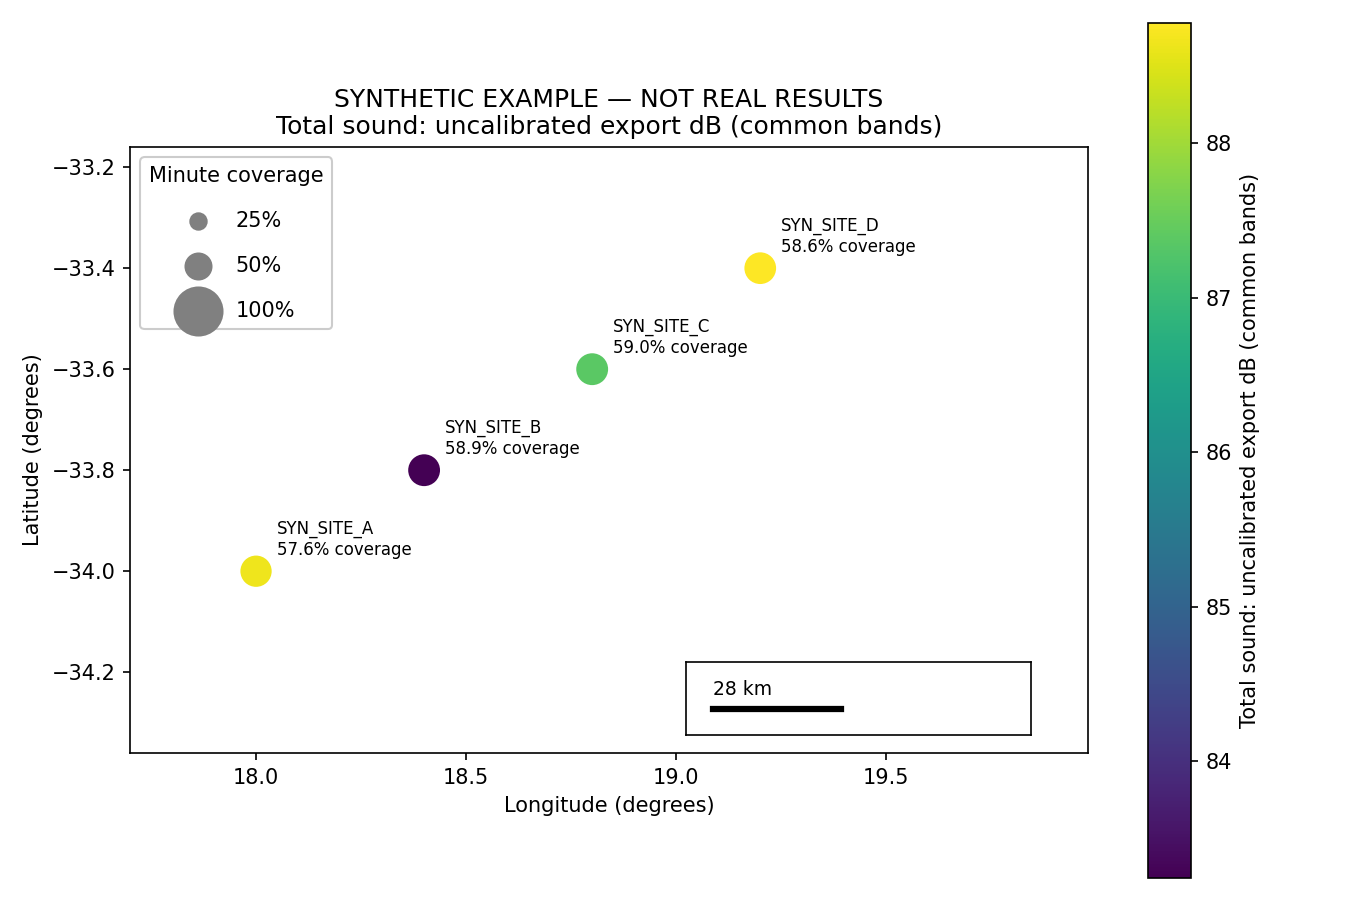
\includegraphics[width=.72\linewidth,height=5.0cm,keepaspectratio]{figures/station_map.png}
\caption{\synthetic{} Invented stations and coordinates. Colour is the median
common-band level in uncalibrated export dB; size/labels encode minute
coverage. These are total-sound proxies, not vessel-specific pressure.}
\end{figure}

\begin{figure}[H]
\centering
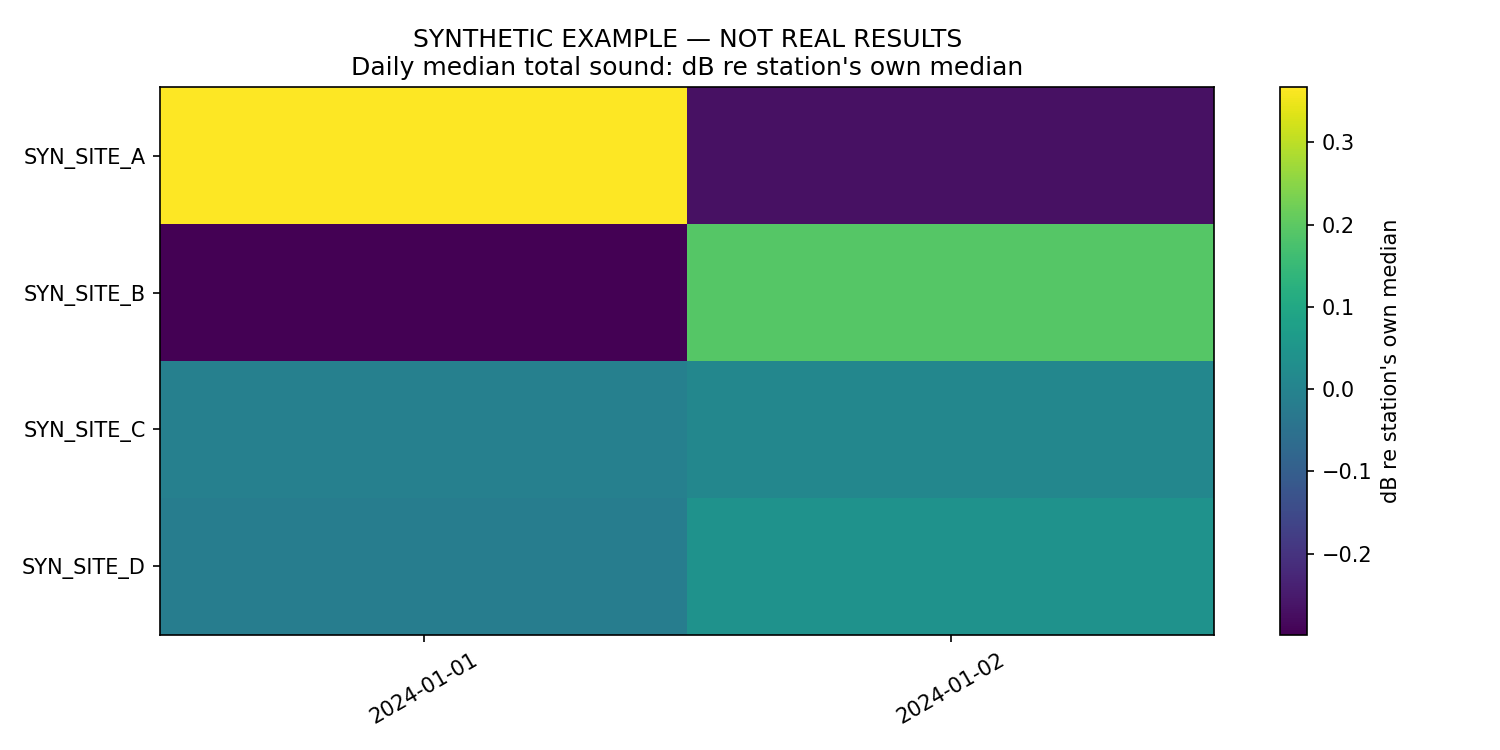
\includegraphics[width=.49\linewidth]{figures/daily_relative.png}\hfill
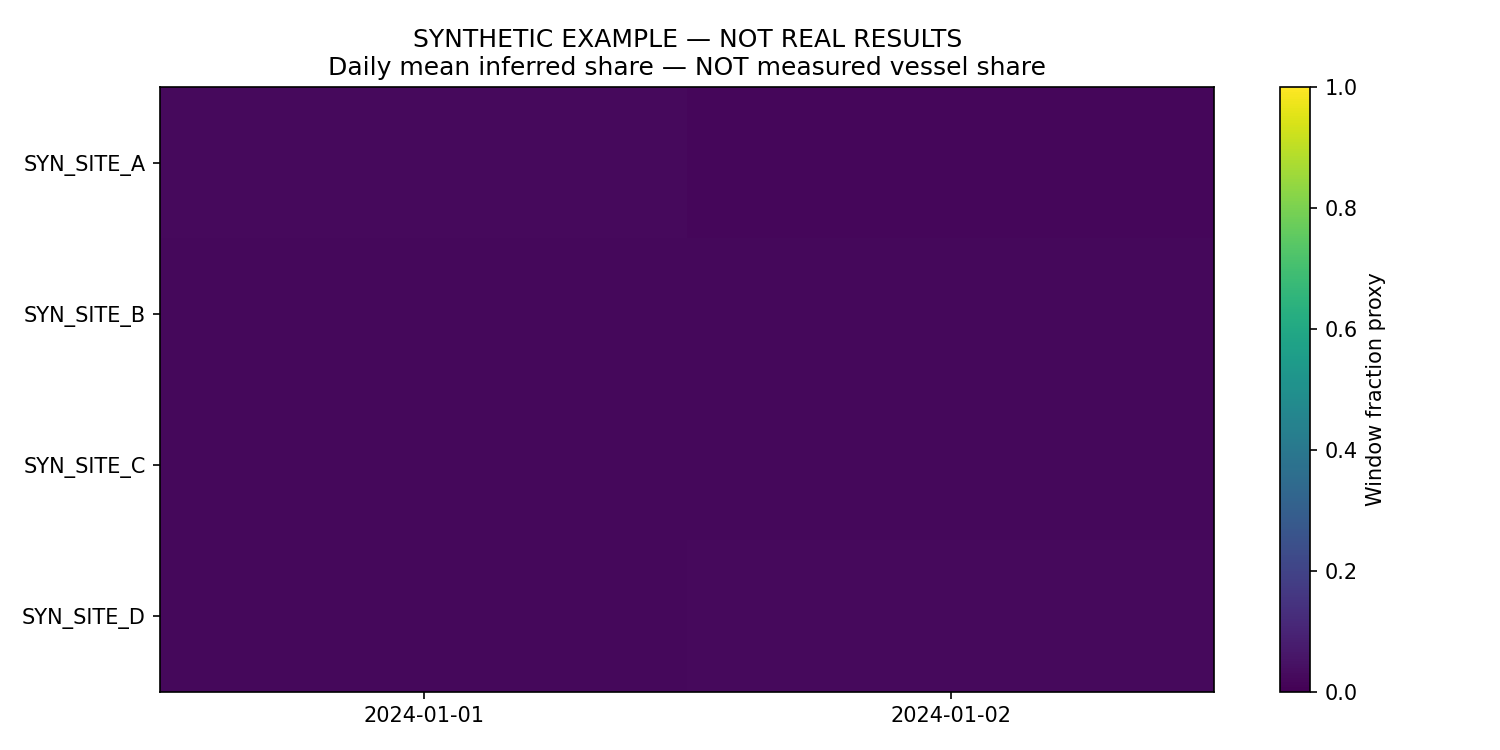
\includegraphics[width=.49\linewidth]{figures/daily_inferred_share.png}
\caption{\synthetic{} Left: station--day median relative level (dB re each
station's median). Right: mean model-inferred added-vessel-like share on
sliding 15-minute windows, stride five minutes. This is a model response to
background sound, \textbf{not a measured natural vessel contribution}.
Overlapping windows are repeated observations, not independent evidence.}
\end{figure}

Total sound, excess energy and inferred added-reference fractions are distinct.
The pipeline also exports a station--day excess-energy heatmap. Without
independent acoustic validation, none supports vessel counts, identities,
sizes, calibrated pressure or causal ecological claims.

\newpage
\section{Interpretability}
LightGBM gain importance identifies split-use contributions to the fitted
regressor. Ridge coefficients describe standardised predictors, including
missing indicators, not original-unit causal effects. TreeSHAP-style
contributions use LightGBM's \texttt{pred\_contrib=True} on training features;
the expected-value column is excluded before averaging absolute contributions.
We sum these means within feature families and explicitly indexed bands.
Group/global effects are retained in family attribution, not arbitrarily
distributed among bands. Correlation can redistribute importance, and
training-distribution explanations do not establish real-data transfer.

\begin{figure}[H]
\centering
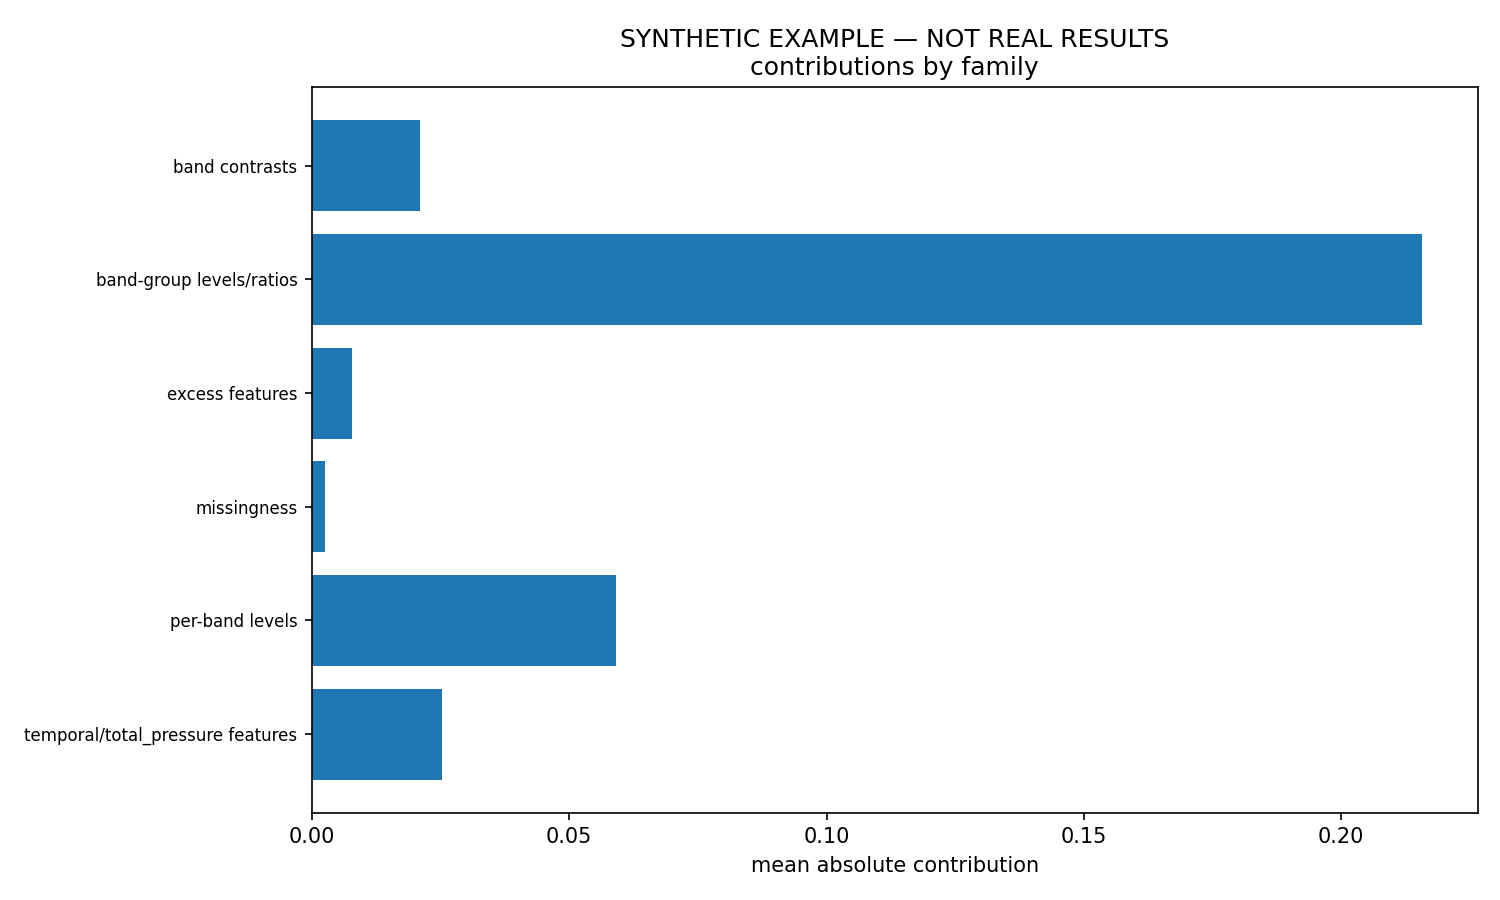
\includegraphics[width=.49\linewidth]{figures/contributions_by_family.png}\hfill
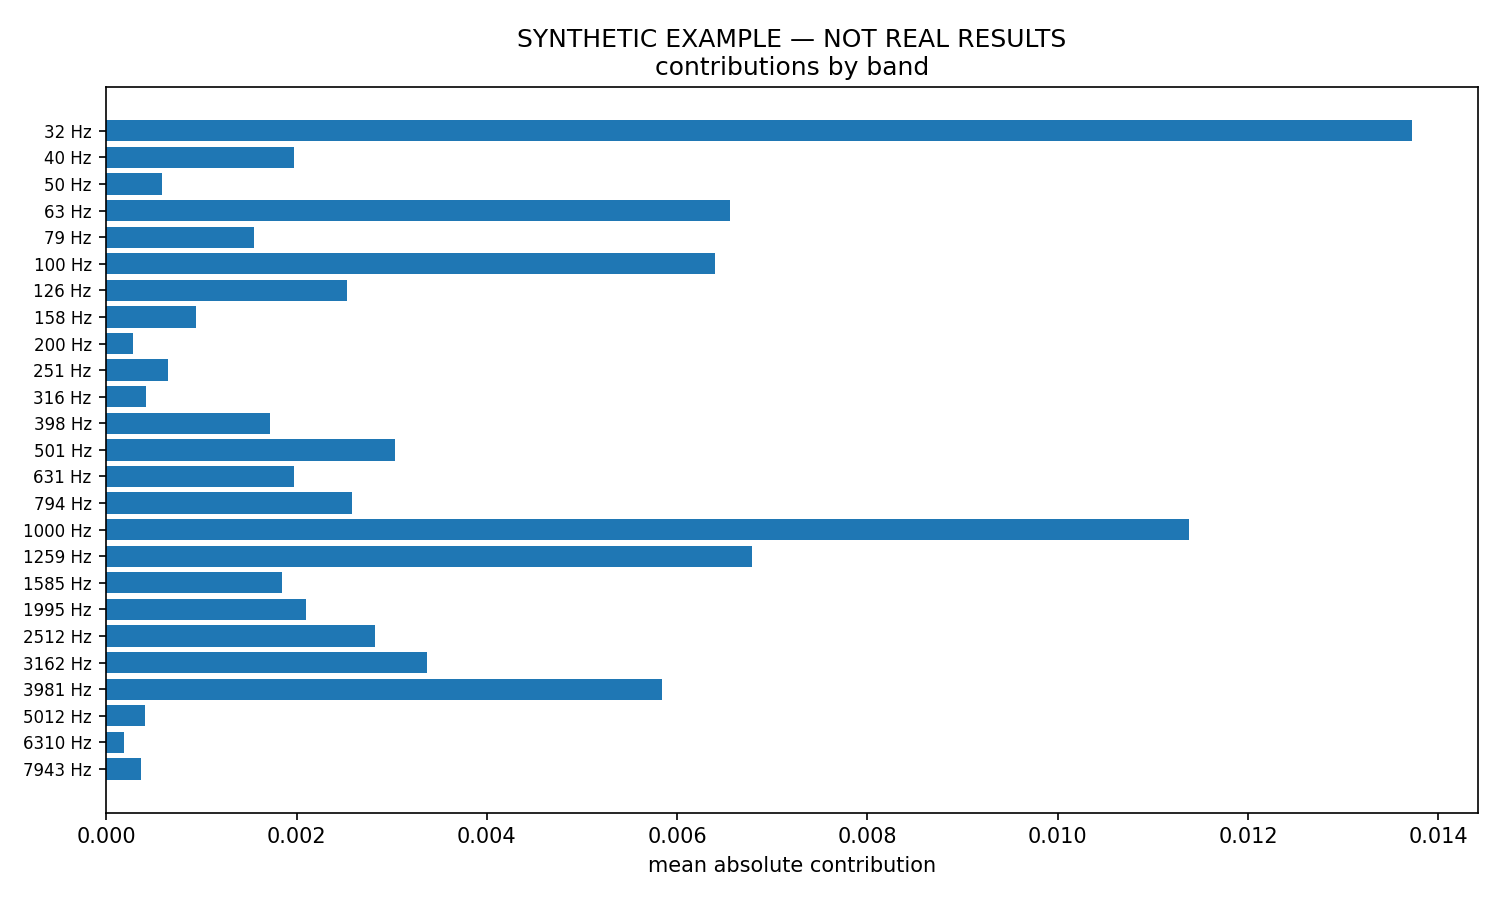
\includegraphics[width=.49\linewidth]{figures/contributions_by_band.png}
\caption{\synthetic{} Mean absolute LightGBM contributions by feature family
(left) and explicitly indexed frequency band (right, centres in Hz).
Contribution magnitudes are in predicted-share units. The band summary
excludes group/global effects and need not total the family summary.}
\end{figure}

\section{Uncertainty and limitations}
\textbf{Synthetic templates are not real passage references.} The challenge
mixes real backgrounds with references derived from recordings, whereas this
experiment invents both. Spectral smoothness, passage timing, reference
ambient floors and the share prior can create shortcuts absent from test
conditions. Adding realistic-looking confounders does not prove realism.
The model may recognise generator artefacts rather than vessels.

\textbf{Domain shift and ambiguity.} Recorders, calibration, biological
activity and sea state vary. Natural vessels already present in backgrounds
are unlabelled. A zero controlled-addition label does not say the window is
vessel-free. Very weak additions, partial passages and high ambient floors
may be indistinguishable. Actual test share and reference distributions are
unknown; good synthetic error need not predict competition performance.
No AIS is used. Future AIS proximity would be weak evidence only, requiring
clock checks and acoustic validation; absent AIS does not mean absent vessels.

The accompanying figure archive includes OOF error-by-share-bin curves with
background-cluster intervals and a diagnostic ROC. Both concern controlled
additions only. Neither error nor AUC estimates reliability on unlabelled
natural vessel activity.

\newpage
\section{Efficiency and reproduction}
\textbf{Synthetic benchmark only:} on an \HardwareCPUs{}-vCPU x86\_64 VM,
training took \TrainSeconds{} s, the full demo \DemoSeconds{} s and the
figure/table workflow \FigureSeconds{} s. The bundle is \ModelBytes{} bytes.
Inference for \HeldoutCount{} examples took \InferenceSeconds{} s with
\InferenceMemory{} MiB peak process RSS; the workflow maximum per-process
RSS was \PeakMemory{} MiB. RSS is a high-water mark including earlier
allocations, not isolated inference allocation or aggregate concurrent RAM.
Values come from \path{tables/metrics_summary.json}; real-release costs
are unmeasured and training is in-memory.

Use Python 3.10 (verified 3.10.12), a venv and \texttt{requirements.txt}.
Seed 42 controls generation/models. LightGBM uses one thread,
\texttt{deterministic=True}, \texttt{force\_row\_wise=True} and seeded randomness.
Cross-platform numerical identity is not guaranteed. Exact direct pins:
{\footnotesizenumpy 1.26.4; pandas 2.2.3; pyarrow 18.1.0; scikit-learn 1.5.2; lightgbm 4.5.0; scipy 1.14.1; matplotlib 3.9.3; joblib 1.4.2; pytest 8.3.4; nbformat 5.10.4; nbconvert 7.16.4; ipykernel 6.29.5; pyparsing 3.2.0.
}

{\footnotesize\begin{verbatim}
python3.10 -m venv .venv
source .venv/bin/activate
pip install -r requirements.txt
python scripts/make_figures.py
bash scripts/build_writeup.sh
pytest -q
\end{verbatim}}
The figure script runs the larger synthetic demo; the build reads JSON macros
and runs \texttt{pdflatex} twice. The notebook defaults to synthetic mode;
real mode requires all input paths and skips evaluation without labels.

\subsection*{Real South African results --- placeholder}
\textbf{No real acoustic results are available.} After the user downloads
the release, Test.csv and sample submission into \texttt{data/}, run these
commands from the repository root (continued lines are shell syntax):
{\footnotesize\begin{verbatim}
python -m src.train --release data/South_African_Real_Acoustics.zip \
  --out-dir models/real --seed 42
python -m src.pressure_map \
  --release data/South_African_Real_Acoustics.zip \
  --model models/real/bundle.joblib --out-dir outputs/real/maps
python -m src.explain --model models/real/bundle.joblib \
  --features models/real/SYNTHETIC_addition_features.parquet \
  --out-dir outputs/real/explanations
python -m src.ablation \
  --features models/real/SYNTHETIC_addition_features.parquet \
  --oof models/real/SYNTHETIC_addition_oof.parquet \
  --out-dir outputs/real/ablations --seed 42
\end{verbatim}}
Training regenerates controlled-addition OOF metrics, not natural ground
truth. Mapping regenerates \path{station_map.png}, \path{daily_relative.png},
\path{daily_inferred_share.png} and \path{daily_excess_energy.png}; explanation
regenerates family/band panels; ablation regenerates the control table.
Review real cases, coverage and clocks before adding separate real panels
and rebuilding. No command can manufacture missing verified real labels.

{\small\textbf{Sources.} Competition Info/Evaluation/Rules and Data tabs,
locally supplied page snapshots; committed source metrics and tables in
\texttt{writeup/tables/}. Future sources: ONC access URL above; HearMyShip
dataset as named on the competition Data tab. No external corpus used.}
\end{document}
